\documentclass[12pt, a4paper,  BCOR=8.25mm, DIV=15]{scrartcl}\usepackage[]{graphicx}\usepackage[]{color}
%% maxwidth is the original width if it is less than linewidth
%% otherwise use linewidth (to make sure the graphics do not exceed the margin)
\makeatletter
\def\maxwidth{ %
  \ifdim\Gin@nat@width>\linewidth
    \linewidth
  \else
    \Gin@nat@width
  \fi
}
\makeatother

\definecolor{fgcolor}{rgb}{0.345, 0.345, 0.345}
\newcommand{\hlnum}[1]{\textcolor[rgb]{0.686,0.059,0.569}{#1}}%
\newcommand{\hlstr}[1]{\textcolor[rgb]{0.192,0.494,0.8}{#1}}%
\newcommand{\hlcom}[1]{\textcolor[rgb]{0.678,0.584,0.686}{\textit{#1}}}%
\newcommand{\hlopt}[1]{\textcolor[rgb]{0,0,0}{#1}}%
\newcommand{\hlstd}[1]{\textcolor[rgb]{0.345,0.345,0.345}{#1}}%
\newcommand{\hlkwa}[1]{\textcolor[rgb]{0.161,0.373,0.58}{\textbf{#1}}}%
\newcommand{\hlkwb}[1]{\textcolor[rgb]{0.69,0.353,0.396}{#1}}%
\newcommand{\hlkwc}[1]{\textcolor[rgb]{0.333,0.667,0.333}{#1}}%
\newcommand{\hlkwd}[1]{\textcolor[rgb]{0.737,0.353,0.396}{\textbf{#1}}}%

\usepackage{framed}
\makeatletter
\newenvironment{kframe}{%
 \def\at@end@of@kframe{}%
 \ifinner\ifhmode%
  \def\at@end@of@kframe{\end{minipage}}%
  \begin{minipage}{\columnwidth}%
 \fi\fi%
 \def\FrameCommand##1{\hskip\@totalleftmargin \hskip-\fboxsep
 \colorbox{shadecolor}{##1}\hskip-\fboxsep
     % There is no \\@totalrightmargin, so:
     \hskip-\linewidth \hskip-\@totalleftmargin \hskip\columnwidth}%
 \MakeFramed {\advance\hsize-\width
   \@totalleftmargin\z@ \linewidth\hsize
   \@setminipage}}%
 {\par\unskip\endMakeFramed%
 \at@end@of@kframe}
\makeatother

\definecolor{shadecolor}{rgb}{.97, .97, .97}
\definecolor{messagecolor}{rgb}{0, 0, 0}
\definecolor{warningcolor}{rgb}{1, 0, 1}
\definecolor{errorcolor}{rgb}{1, 0, 0}
\newenvironment{knitrout}{}{} % an empty environment to be redefined in TeX

\usepackage{alltt}
\usepackage[utf8]{inputenc}
\usepackage{newfloat}
\DeclareFloatingEnvironment[name={Supplementary Figure}]{suppfigure}

\newenvironment{itemizz}%
  {\begin{itemize}%
    \setlength{\itemsep}{2pt}%
    \setlength{\parskip}{2pt}}%
  {\end{itemize}}

\newcommand{\txtt}[1]{{\texttt{#1}}}
\IfFileExists{upquote.sty}{\usepackage{upquote}}{}
\begin{document}
%\VignetteEngine{knitr::knitr}
%\VignetteIndexEntry{Examples (Set 5)}



\title{5: Examples }
\author{John H Maindonald}
\maketitle

\begin{knitrout}
\definecolor{shadecolor}{rgb}{0.969, 0.969, 0.969}\color{fgcolor}\begin{kframe}
\begin{alltt}
\hlstd{fig5.1A} \hlkwb{<-} \hlkwa{function}\hlstd{()\{}
\hlcom{## ---- brain-bodyA ----}
\hlkwd{library}\hlstd{(MASS)}
\hlkwd{plot}\hlstd{(brain} \hlopt{~} \hlstd{body,} \hlkwc{data}\hlstd{=mammals)}
\hlkwd{mtext}\hlstd{(}\hlkwc{side}\hlstd{=}\hlnum{3}\hlstd{,} \hlkwc{line}\hlstd{=}\hlnum{0.5}\hlstd{,} \hlkwc{adj}\hlstd{=}\hlnum{0}\hlstd{,} \hlstr{"A: Unlogged data"}\hlstd{)}
\hlstd{\}}
\hlstd{fig5.1B} \hlkwb{<-} \hlkwa{function}\hlstd{()\{}
\hlcom{## ---- brain-bodyB ----}
\hlkwd{plot}\hlstd{(brain} \hlopt{~} \hlstd{body,} \hlkwc{data}\hlstd{=mammals,} \hlkwc{log}\hlstd{=}\hlstr{"xy"}\hlstd{)}
\hlkwd{mtext}\hlstd{(}\hlkwc{side}\hlstd{=}\hlnum{3}\hlstd{,} \hlkwc{line}\hlstd{=}\hlnum{0.5}\hlstd{,} \hlkwc{adj}\hlstd{=}\hlnum{0}\hlstd{,}
      \hlstr{"B: Log scales (both axes)"}\hlstd{)}
\hlstd{\}}
\hlstd{fig5.1} \hlkwb{<-} \hlkwa{function}\hlstd{()\{}
\hlstr{"Run the separate functions fig5.1A() and fig5.1B()."}
\hlstd{\}}
\end{alltt}
\end{kframe}
\end{knitrout}

\begin{knitrout}
\definecolor{shadecolor}{rgb}{0.969, 0.969, 0.969}\color{fgcolor}\begin{kframe}
\begin{alltt}
\hlstd{fig5.2} \hlkwb{<-} \hlkwa{function}\hlstd{()\{}
\hlcom{## ---- plot-trees ----}
\hlcom{## Code used for the plot}
\hlkwd{plot}\hlstd{(trees,} \hlkwc{cex.labels}\hlstd{=}\hlnum{1.5}\hlstd{)}
  \hlcom{# Calls pairs(trees)}
\hlstd{\}}
\end{alltt}
\end{kframe}
\end{knitrout}

\begin{knitrout}
\definecolor{shadecolor}{rgb}{0.969, 0.969, 0.969}\color{fgcolor}\begin{kframe}
\begin{alltt}
\hlstd{fig5.3} \hlkwb{<-} \hlkwa{function}\hlstd{()\{}
\hlcom{## ---- trackVSroad ----}
\hlcom{## Code}
\hlkwd{library}\hlstd{(lattice)}
\hlkwd{xyplot}\hlstd{(Time} \hlopt{~} \hlstd{Distance,} \hlkwc{scales}\hlstd{=}\hlkwd{list}\hlstd{(}\hlkwc{tck}\hlstd{=}\hlnum{0.5}\hlstd{),}
       \hlkwc{groups}\hlstd{=roadORtrack,} \hlkwc{data}\hlstd{=DAAG}\hlopt{::}\hlstd{worldRecords,}
       \hlkwc{auto.key}\hlstd{=}\hlkwd{list}\hlstd{(}\hlkwc{columns}\hlstd{=}\hlnum{2}\hlstd{),} \hlkwc{aspect}\hlstd{=}\hlnum{1}\hlstd{)}
\hlcom{## On a a colour device the default is to use}
\hlcom{## different colours, not different symbols,}
\hlcom{## to distinguish groups.}
\hlstd{\}}
\end{alltt}
\end{kframe}
\end{knitrout}

\begin{knitrout}
\definecolor{shadecolor}{rgb}{0.969, 0.969, 0.969}\color{fgcolor}\begin{kframe}
\begin{alltt}
\hlstd{fig5.4A} \hlkwb{<-} \hlkwa{function}\hlstd{()\{}
\hlcom{## ---- wrTimesA ----}
\hlcom{## Code for Left panel}
\hlstd{parset} \hlkwb{<-} \hlkwd{list}\hlstd{(}\hlkwc{layout.widths}\hlstd{=}\hlkwd{list}\hlstd{(}\hlkwc{left.padding}\hlstd{=}\hlnum{2.5}\hlstd{,}
                                  \hlkwc{right.padding}\hlstd{=}\hlnum{2.5}\hlstd{))}
\hlkwd{xyplot}\hlstd{(}\hlkwd{log}\hlstd{(Time)} \hlopt{~} \hlkwd{log}\hlstd{(Distance),}
       \hlkwc{groups}\hlstd{=roadORtrack,} \hlkwc{data}\hlstd{=DAAG}\hlopt{::}\hlstd{worldRecords,}
       \hlkwc{scales}\hlstd{=}\hlkwd{list}\hlstd{(}\hlkwc{tck}\hlstd{=}\hlnum{0.5}\hlstd{),}
       \hlkwc{par.settings}\hlstd{=parset,}
       \hlkwc{auto.key}\hlstd{=}\hlkwd{list}\hlstd{(}\hlkwc{columns}\hlstd{=}\hlnum{2}\hlstd{),} \hlkwc{aspect}\hlstd{=}\hlnum{1}\hlstd{)}
\hlstd{\}}
\hlstd{fig5.4B} \hlkwb{<-} \hlkwa{function}\hlstd{()\{}
\hlcom{## ---- wrTimesB ----}
\hlcom{## Right panel}
\hlkwd{xyplot}\hlstd{(Time} \hlopt{~} \hlstd{Distance,} \hlkwc{groups}\hlstd{=roadORtrack,}
       \hlkwc{data}\hlstd{=DAAG}\hlopt{::}\hlstd{worldRecords,}
       \hlkwc{scales}\hlstd{=}\hlkwd{list}\hlstd{(}\hlkwc{log}\hlstd{=}\hlnum{10}\hlstd{,} \hlkwc{tck}\hlstd{=}\hlnum{0.5}\hlstd{),}
       \hlkwc{auto.key}\hlstd{=}\hlkwd{list}\hlstd{(}\hlkwc{columns}\hlstd{=}\hlnum{2}\hlstd{),} \hlkwc{aspect}\hlstd{=}\hlnum{1}\hlstd{)}
\hlstd{\}}
\hlstd{fig5.4} \hlkwb{<-} \hlkwa{function}\hlstd{()\{}
\hlstr{"Run the separate functions fig5.4A() and fig5.4B()."}
\hlstd{\}}
\end{alltt}
\end{kframe}
\end{knitrout}

\begin{knitrout}
\definecolor{shadecolor}{rgb}{0.969, 0.969, 0.969}\color{fgcolor}\begin{kframe}
\begin{alltt}
\hlstd{suppfig5.1} \hlkwb{<-} \hlkwa{function}\hlstd{()\{}
\hlcom{## ---- timevsDist ----}
\hlkwd{plot}\hlstd{(}\hlkwd{log}\hlstd{(Time)} \hlopt{~} \hlkwd{log}\hlstd{(Distance),}
     \hlkwc{data} \hlstd{= DAAG}\hlopt{::}\hlstd{worldRecords)}
\hlkwd{abline}\hlstd{(worldrec.lm)}
\hlstd{\}}
\end{alltt}
\end{kframe}
\end{knitrout}

\begin{knitrout}
\definecolor{shadecolor}{rgb}{0.969, 0.969, 0.969}\color{fgcolor}\begin{kframe}
\begin{alltt}
\hlstd{fig5.5} \hlkwb{<-} \hlkwa{function}\hlstd{()\{}
\hlcom{## ---- diag12 ----}
\hlkwd{plot}\hlstd{(worldrec.lm,} \hlkwc{which}\hlstd{=}\hlkwd{c}\hlstd{(}\hlnum{1}\hlstd{,}\hlnum{5}\hlstd{),} \hlkwc{sub.caption}\hlstd{=}\hlkwd{rep}\hlstd{(}\hlstr{""}\hlstd{,}\hlnum{2}\hlstd{))}
\hlstd{\}}
\end{alltt}
\end{kframe}
\end{knitrout}



\begin{knitrout}
\definecolor{shadecolor}{rgb}{0.969, 0.969, 0.969}\color{fgcolor}\begin{kframe}
\begin{alltt}
\hlstd{fig5.6A} \hlkwb{<-} \hlkwa{function}\hlstd{()\{}
\hlcom{## ---- nihills-spmA ----}
\hlcom{## Scatterplot matrix; unlogged data}
\hlkwd{library}\hlstd{(lattice)}
\hlkwd{splom}\hlstd{(}\hlopt{~}\hlstd{DAAG}\hlopt{::}\hlstd{nihills,}  \hlkwc{lower.panel}\hlstd{=showcorr,} \hlkwc{xlab}\hlstd{=}\hlstr{""}\hlstd{)}
\hlstd{\}}
\hlstd{fig5.6B} \hlkwb{<-} \hlkwa{function}\hlstd{()\{}
\hlcom{## ---- nihills-spmB ----}
\hlstd{lognihills} \hlkwb{<-} \hlkwd{log}\hlstd{(DAAG}\hlopt{::}\hlstd{nihills)}
\hlkwd{names}\hlstd{(lognihills)} \hlkwb{<-} \hlkwd{paste0}\hlstd{(}\hlstr{"l"}\hlstd{,} \hlkwd{names}\hlstd{(DAAG}\hlopt{::}\hlstd{nihills))}
\hlcom{## Scatterplot matrix; log scales}
\hlkwd{splom}\hlstd{(}\hlopt{~} \hlstd{lognihills,} \hlkwc{lower.panel}\hlstd{=showcorr,} \hlkwc{xlab}\hlstd{=}\hlstr{""}\hlstd{)}
\hlstd{\}}
\hlstd{fig5.6} \hlkwb{<-} \hlkwa{function}\hlstd{()\{}
  \hlkwd{print}\hlstd{(}\hlstr{"Run the separate functions fig5.6A() and fig5.6B()"}\hlstd{)}
\hlstd{\}}
\end{alltt}
\end{kframe}
\end{knitrout}

\begin{knitrout}
\definecolor{shadecolor}{rgb}{0.969, 0.969, 0.969}\color{fgcolor}\begin{kframe}
\begin{alltt}
\hlstd{fig5.7} \hlkwb{<-} \hlkwa{function}\hlstd{()\{}
\hlcom{## Requires ggplot2}
\hlstd{tomato} \hlkwb{<-} \hlkwd{within}\hlstd{(DAAG}\hlopt{::}\hlstd{tomato, trt} \hlkwb{<-} \hlkwd{relevel}\hlstd{(trt,} \hlkwc{ref}\hlstd{=}\hlstr{"water only"}\hlstd{))}
\hlstd{ggplot2}\hlopt{::}\hlkwd{quickplot}\hlstd{(weight, trt,} \hlkwc{data}\hlstd{=DAAG}\hlopt{::}\hlstd{tomato,} \hlkwc{xlab}\hlstd{=}\hlstr{"Weight (g)"}\hlstd{,} \hlkwc{ylab}\hlstd{=}\hlstr{""}\hlstd{)}
\hlstd{\}}
\end{alltt}
\end{kframe}
\end{knitrout}

\begin{knitrout}
\definecolor{shadecolor}{rgb}{0.969, 0.969, 0.969}\color{fgcolor}\begin{kframe}
\begin{alltt}
\hlstd{fig5.8} \hlkwb{<-} \hlkwa{function}\hlstd{()\{}
\hlstd{opar} \hlkwb{<-} \hlkwd{par}\hlstd{(}\hlkwc{xpd}\hlstd{=}\hlnum{TRUE}\hlstd{,} \hlkwc{mar}\hlstd{=}\hlkwd{c}\hlstd{(}\hlnum{3.1}\hlstd{,}\hlnum{3.1}\hlstd{,}\hlnum{0.6}\hlstd{,}\hlnum{3.6}\hlstd{),} \hlkwc{mgp}\hlstd{=}\hlkwd{c}\hlstd{(}\hlnum{2.25}\hlstd{,} \hlnum{0.5}\hlstd{,} \hlnum{0}\hlstd{))}
\hlkwd{with}\hlstd{(DAAG}\hlopt{::}\hlstd{rice,} \hlkwd{interaction.plot}\hlstd{(}\hlkwc{x.factor}\hlstd{=fert,}
                            \hlkwc{trace.factor}\hlstd{=variety,}
                            \hlstd{ShootDryMass,}
                            \hlkwc{cex.lab}\hlstd{=}\hlnum{1.4}\hlstd{))}
\hlkwd{par}\hlstd{(opar)}
\hlstd{\}}
\end{alltt}
\end{kframe}
\end{knitrout}

\begin{knitrout}
\definecolor{shadecolor}{rgb}{0.969, 0.969, 0.969}\color{fgcolor}\begin{kframe}
\begin{alltt}
\hlstd{fig5.9} \hlkwb{<-} \hlkwa{function}\hlstd{()\{}
\hlcom{## ---- MDBrainfall ----}
\hlcom{## Code}
\hlkwd{plot}\hlstd{(mdbRain} \hlopt{~} \hlstd{Year,} \hlkwc{data}\hlstd{=DAAG}\hlopt{::}\hlstd{bomregions2012)}
\hlcom{## Calculate and plot curve showing long-term trend}
\hlkwd{with}\hlstd{(DAAG}\hlopt{::}\hlstd{bomregions2012,} \hlkwd{lines}\hlstd{(}\hlkwd{lowess}\hlstd{(mdbRain} \hlopt{~} \hlstd{Year,}
                           \hlkwc{f}\hlstd{=}\hlnum{2}\hlopt{/}\hlnum{3}\hlstd{),} \hlkwc{lty}\hlstd{=}\hlnum{2}\hlstd{))}
\hlcom{## Calculate and plot curve of short-term trends}
\hlkwd{with}\hlstd{(DAAG}\hlopt{::}\hlstd{bomregions2012,}
     \hlkwd{lines}\hlstd{(}\hlkwd{lowess}\hlstd{(mdbRain} \hlopt{~} \hlstd{Year,} \hlkwc{f}\hlstd{=}\hlnum{0.1}\hlstd{),} \hlkwc{lty}\hlstd{=}\hlnum{1}\hlstd{))}
\hlstd{\}}
\end{alltt}
\end{kframe}
\end{knitrout}

\begin{knitrout}
\definecolor{shadecolor}{rgb}{0.969, 0.969, 0.969}\color{fgcolor}\begin{kframe}
\begin{alltt}
\hlstd{figset5} \hlkwb{<-} \hlkwa{function}\hlstd{()\{}
    \hlkwa{if}\hlstd{(}\hlopt{!}\hlkwd{requireNamespace}\hlstd{(}\hlstr{'DAAG'}\hlstd{))}\hlkwd{stop}\hlstd{(}\hlstr{'DAAG must be installed'}\hlstd{)}
  \hlkwa{if}\hlstd{(}\hlopt{!}\hlkwd{requireNamespace}\hlstd{(}\hlstr{'ggplot2'}\hlstd{))}\hlkwd{stop}\hlstd{(}\hlstr{'ggplot2 must be installed'}\hlstd{)}
  \hlstd{\}}
\end{alltt}
\end{kframe}
\end{knitrout}

\begin{knitrout}
\definecolor{shadecolor}{rgb}{0.969, 0.969, 0.969}\color{fgcolor}\begin{kframe}
\begin{alltt}
\hlkwd{figset5}\hlstd{()}
\end{alltt}


{\ttfamily\noindent\itshape\color{messagecolor}{Loading required namespace: DAAG\\Loading required namespace: ggplot2}}\begin{alltt}
\hlkwa{if}\hlstd{(}\hlopt{!}\hlkwd{exists}\hlstd{(}\hlstr{"worldrec.lm"}\hlstd{))\{}
    \hlstd{worldrec.lm} \hlkwb{<-} \hlkwd{lm}\hlstd{(}\hlkwd{log}\hlstd{(Time)} \hlopt{~} \hlkwd{log}\hlstd{(Distance),}
                      \hlkwc{data}\hlstd{=DAAG}\hlopt{::}\hlstd{worldRecords)}
\hlstd{\}}
\end{alltt}
\end{kframe}
\end{knitrout}


\begin{figure}
\begin{knitrout}
\definecolor{shadecolor}{rgb}{0.969, 0.969, 0.969}\color{fgcolor}

{\centering 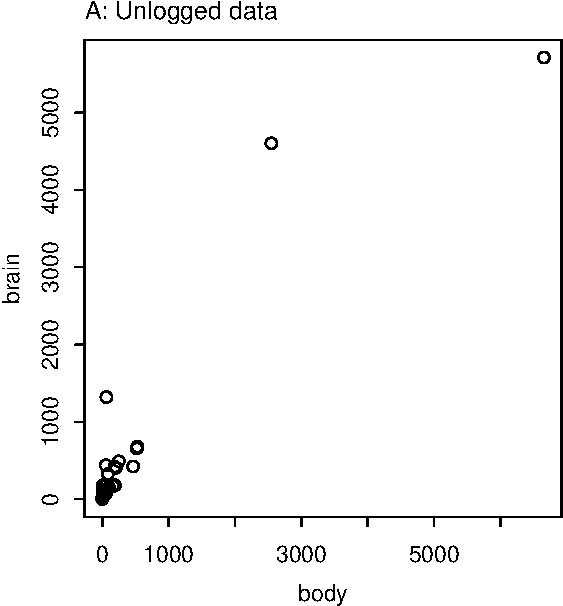
\includegraphics[width=0.47\textwidth]{figs/glm-fig5_1e-1} 
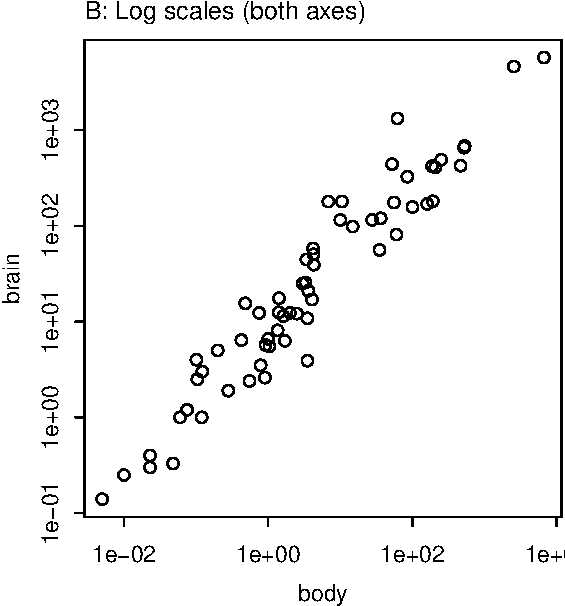
\includegraphics[width=0.47\textwidth]{figs/glm-fig5_1e-2} 

}



\end{knitrout}
\caption{Brain weight (g) versus Body weight (kg), for 62 species of mammal.
Panel A plots the unlogged data, while Panel B has log scales are used for
both axes. Notice that, in Panel B, the scales are
  labeled in the original (unlogged) units.
  \label{fig:Animals}}
\end{figure}

\begin{figure}
\begin{minipage}[c]{0.525\textwidth}
\fbox{\parbox{\textwidth}{{\bf Interpreting Scatterplot Matrices:}\\[4pt]
For identifying the axes for each panel
\begin{itemizz}
\item[-] look across the row to the diagonal to identify the variable on
 the vertical axis.
\item[-] look up or down the column to the diagonal for the
  variable on the horizontal axis.
\end{itemizz}
Each below diagonal panel is the mirror image of the
corresponding above diagonal panel.
}}
\vspace*{6pt}
\end{minipage}
\begin{minipage}[c]{0.46\textwidth}
\begin{knitrout}
\definecolor{shadecolor}{rgb}{0.969, 0.969, 0.969}\color{fgcolor}\begin{kframe}
\begin{alltt}
\hlkwd{fig5.2}\hlstd{()}
\end{alltt}
\end{kframe}

{\centering 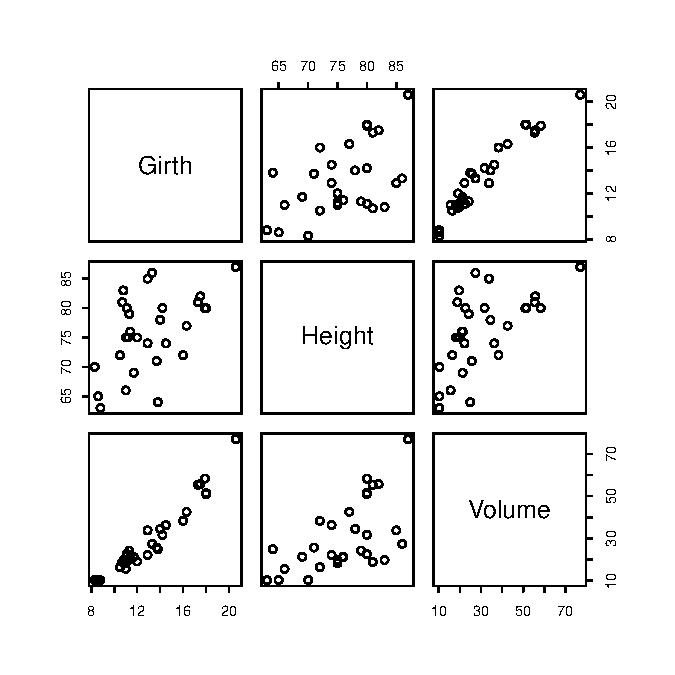
\includegraphics[width=0.97\textwidth]{figs/glm-fig5_2e-1} 

}



\end{knitrout}
\end{minipage}
\caption{Scatterplot matrix for the \txtt{trees} data, obtained
  using the default \txtt{plot()} method for data frames.  The
  scatterplot matrix is a graphical counterpart of the correlation
  matrix.\label{fig:trees}}
\end{figure}

\begin{figure}
\begin{knitrout}
\definecolor{shadecolor}{rgb}{0.969, 0.969, 0.969}\color{fgcolor}\begin{kframe}
\begin{alltt}
\hlkwd{fig5.3}\hlstd{()}
\end{alltt}
\end{kframe}

{\centering 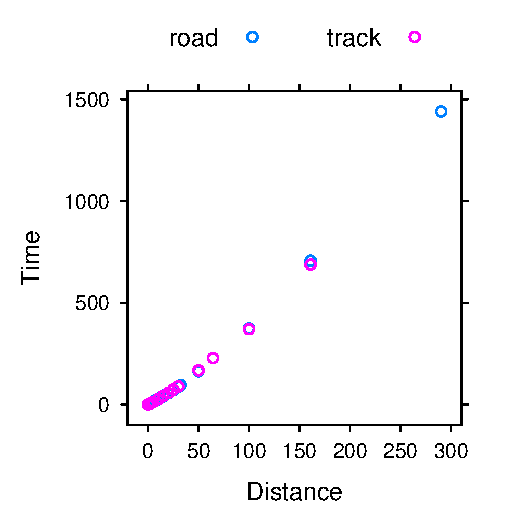
\includegraphics[width=0.6\textwidth]{figs/glm-fig5_3e-1} 

}



\end{knitrout}
\caption{World record times versus distance, for field and road
  events.\label{fig:wrnolog}}
\end{figure}

\begin{figure}
\begin{knitrout}
\definecolor{shadecolor}{rgb}{0.969, 0.969, 0.969}\color{fgcolor}\begin{kframe}
\begin{alltt}
\hlkwd{fig5.4A}\hlstd{()}
\hlkwd{fig5.4B}\hlstd{()}
\end{alltt}
\end{kframe}

{\centering 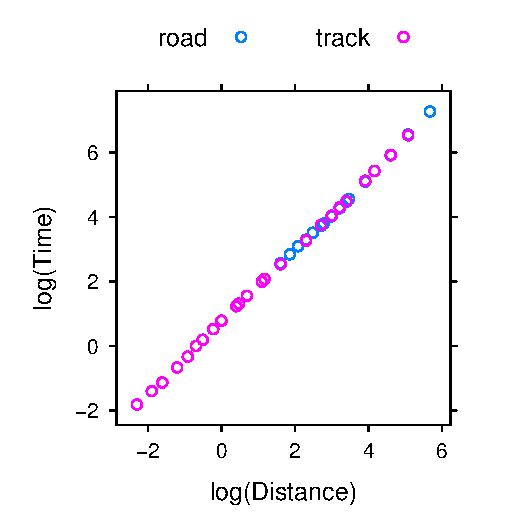
\includegraphics[width=0.47\textwidth]{figs/glm-fig5_4e-1} 
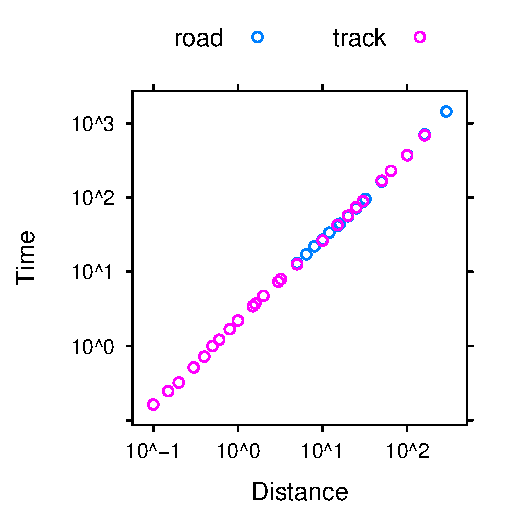
\includegraphics[width=0.47\textwidth]{figs/glm-fig5_4e-2} 

}



\end{knitrout}
\caption{World record times versus distance, for field and road
  events, using logarithmic scales.  The left panel uses labels on
  scales of $\log_e$, while in the right panel, labeling is in the
  orginal units, expressed as powers of 10.}
\label{fig:wrlog}
\end{figure}

\begin{suppfigure}
\begin{knitrout}
\definecolor{shadecolor}{rgb}{0.969, 0.969, 0.969}\color{fgcolor}\begin{kframe}
\begin{alltt}
\hlkwd{suppfig5.1}\hlstd{()}
\end{alltt}
\end{kframe}

{\centering 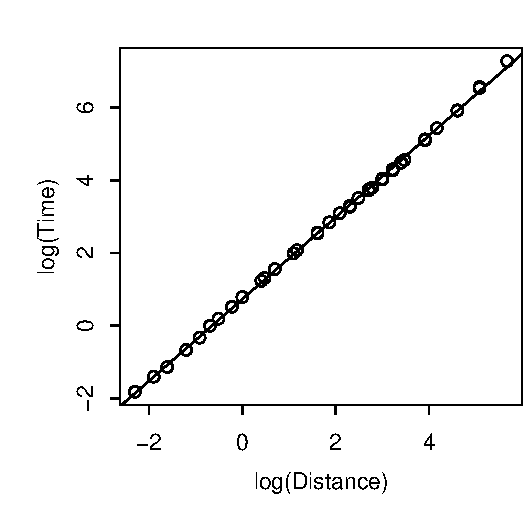
\includegraphics[width=0.47\textwidth]{figs/glm-suppfig5_1e-1} 

}



\end{knitrout}
\caption{log(time) versus log(distance), with a fitted line.}
\end{suppfigure}

\begin{figure}
\begin{knitrout}
\definecolor{shadecolor}{rgb}{0.969, 0.969, 0.969}\color{fgcolor}\begin{kframe}
\begin{alltt}
\hlkwd{fig5.5}\hlstd{()}
\end{alltt}
\end{kframe}

{\centering 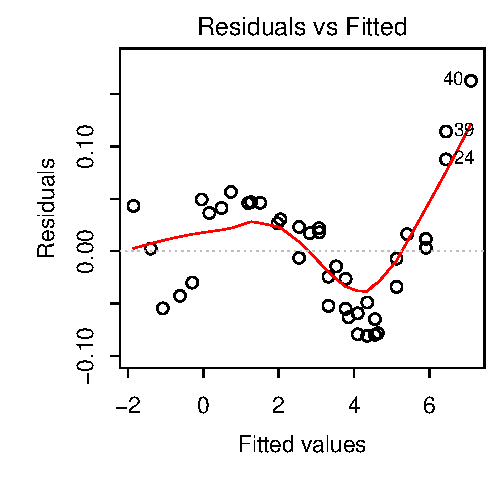
\includegraphics[width=0.47\textwidth]{figs/glm-fig5_5e-1} 
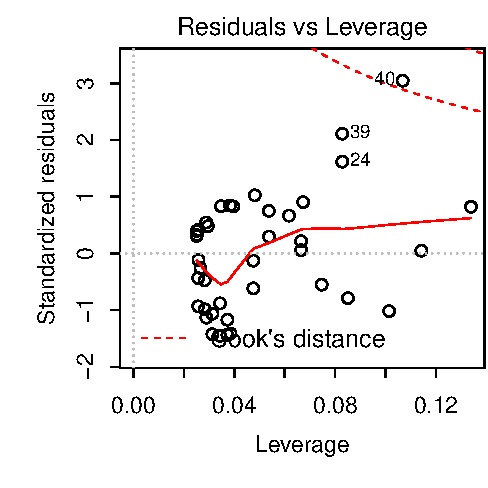
\includegraphics[width=0.47\textwidth]{figs/glm-fig5_5e-2} 

}



\end{knitrout}
      \caption{First and last of the default diagnostic plots, from the
        linear model for log(record time) versus log(distance), for
        field and road events.}
\label{fig:wr-diag}
\end{figure}

\begin{figure}
\vspace*{-6pt}
\begin{knitrout}
\definecolor{shadecolor}{rgb}{0.969, 0.969, 0.969}\color{fgcolor}\begin{kframe}
\begin{alltt}
\hlkwd{fig5.6A}\hlstd{()}
\hlkwd{fig5.6B}\hlstd{()}
\end{alltt}
\end{kframe}

{\centering 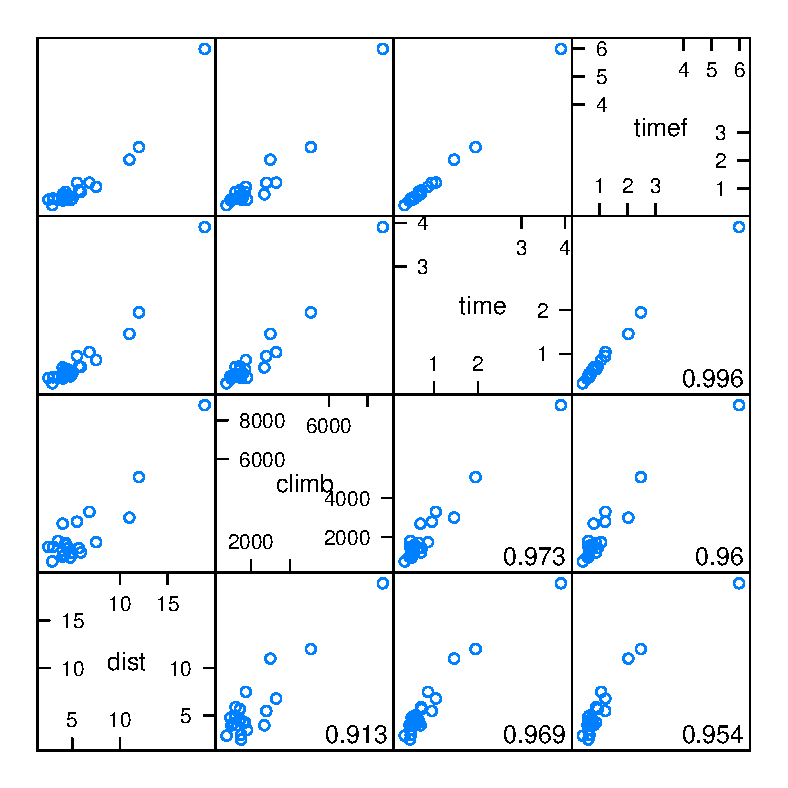
\includegraphics[width=0.47\textwidth]{figs/glm-fig5_6e-1} 
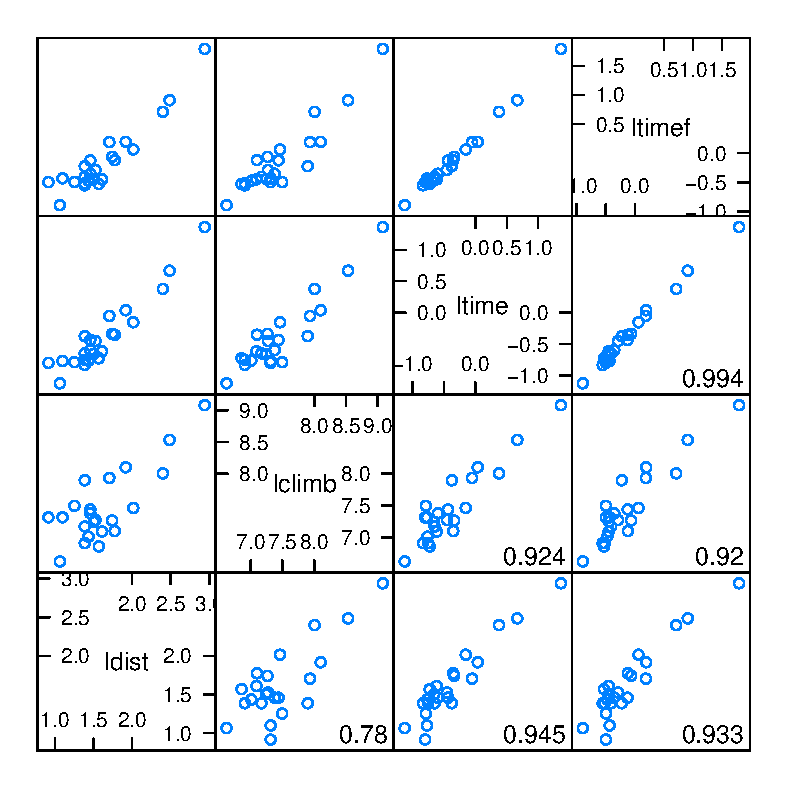
\includegraphics[width=0.47\textwidth]{figs/glm-fig5_6e-2} 

}



\end{knitrout}
\caption{Scatterplot matrices for the Northern Ireland mountain racing
  data. The left panel is for the unlogged data, while the right panel is
for the logged data.  Code has been added that shows the correlations,
in the lower panel.\label{fig:nimra}}
\end{figure}

\begin{figure}
\vspace*{-6pt}
\begin{knitrout}
\definecolor{shadecolor}{rgb}{0.969, 0.969, 0.969}\color{fgcolor}

{\centering 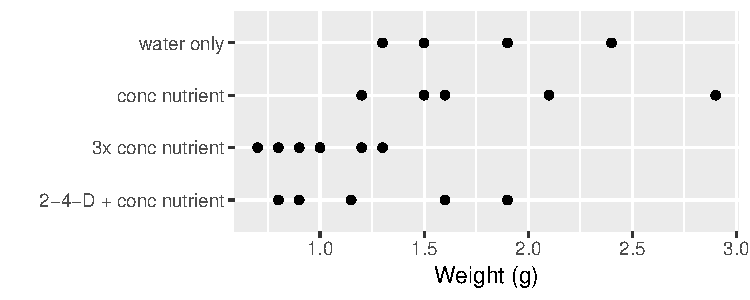
\includegraphics[width=0.98\textwidth]{figs/glm-fig5_7e-1} 

}



\end{knitrout}
\caption{Weights (g) of tomato plants grown under four different
  treatments.\label{fig:Tomato}}
\end{figure}

\begin{figure}
\begin{knitrout}
\definecolor{shadecolor}{rgb}{0.969, 0.969, 0.969}\color{fgcolor}

{\centering 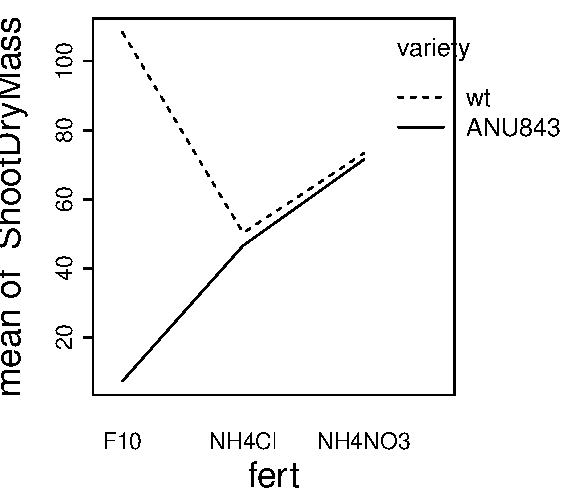
\includegraphics[width=0.55\textwidth]{figs/glm-fig5_8e-1} 

}



\end{knitrout}
    \caption{Interaction plot for the terms \txtt{fert} and
      \txtt{variety}, with \txtt{ShootDryMass} as the dependent
      variable. Notice that for fertilizer F10, there is a huge
      variety difference in the response. For the other fertilizers,
      there is no difference of consequence.\label{fig:rice-interact}}
\end{figure}


\begin{figure}
\begin{knitrout}
\definecolor{shadecolor}{rgb}{0.969, 0.969, 0.969}\color{fgcolor}\begin{kframe}
\begin{alltt}
\hlkwd{fig5.9}\hlstd{()}
\end{alltt}
\end{kframe}

{\centering 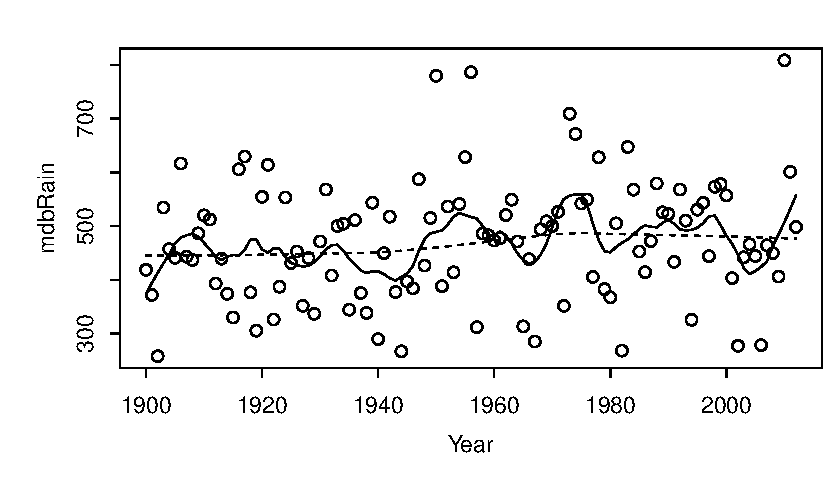
\includegraphics[width=0.65\textwidth]{figs/glm-fig5_9e-1} 

}



\end{knitrout}
\caption{Annual rainfall in the Australian Murray-Darling Basin.
by year.  The \txtt{lowess()} function is used to
The dashed curve with \txtt{f=2/3} captures the
overall trend, while the solid curve with \txtt{f=0.1}
captures trends on a scale of around eleven years. (10\% of the 113 year
range from 1900 to 2012 is a little more than 11 years.)\label{fig:mdbRain}}
\end{figure}

\end{document}
